\documentclass{article}
\usepackage{graphicx}
\usepackage{hyperref}
\usepackage{amsmath}
\usepackage{iclr2024_conference,times}
\iclrfinalcopy
\begin{document}

\title{A Foundational Model for Intelligent Document Processing}
\author{Dr. Arijit Das, ERGO Group AG}
\maketitle

\begin{abstract}
    The rapid advancement in large language models (LLMs) has enabled new capabilities for handling complex, multi-modal data. This paper presents a multi-modal foundation model designed for intelligent document processing, integrating advanced text and image encoders. Leveraging techniques from BEITv2, LLM2Vec, and LongLoRA, our model efficiently handles extended contexts and structured information. The image encoder employs a Vision Transformer (ViT) pre-trained with BEITv2, while the text encoder utilizes a pre-trained LLM, adapted with the LLM2Vec approach for robust text encoding. A multiway transformer integrates the embeddings, facilitating efficient cross-modal attention. The model is pre-trained on large datasets, including IDL-WDS and PDFa-eng-WDS, and fine-tuned on specific tasks with datasets like PubTables-1M and PubLayNet. Our methodology includes a prompt-based fine-tuning strategy, enhancing the model's versatility across various downstream tasks, such as document classification and named entity recognition. Comprehensive experiments demonstrate the model's robust performance and set a new standard for processing multi-modal documents with extended contexts.
\end{abstract}

\section{Introduction}

The rapid advancement in large language models (LLMs) has opened new possibilities for handling complex, multi-modal data. In this paper, we introduce a multi-modal foundation model capable of processing both document images and their Optical Character Recognition (OCR) outputs in JSON format. Our model integrates advanced text and image encoders, incorporating techniques from BEITv2, LLM2Vec, and LongLoRA to handle extended contexts and efficiently process structured information.

For the image encoder, we leverage a Vision Transformer (ViT) model, pre-trained using the BEITv2 approach. Instead of generating image patches directly, the model predicts CLIP embeddings of those patches, enhancing its capability to understand visual content. The text encoder utilizes a pre-trained LLM, such as Llama3 or Mistral, adapted using the LLM2Vec approach. This adaptation includes enabling bidirectional attention, masked next token prediction (MNTP), and unsupervised contrastive learning using the SimCSE technique. These modifications transform the decoder-only LLM into a robust text encoder capable of handling the structured nature of OCR outputs.

We further extend the context window of our model using LongLoRA, which combines Shifted Sparse Attention (S2-Attn) for computational efficiency during fine-tuning and parameter-efficient techniques to manage embeddings and normalization layers effectively. This allows our model to handle significantly larger context sizes without a proportional increase in computational resources, demonstrating strong empirical results on various tasks.

Our model is pre-trained on large datasets such as IDL-WDS and PDFa-eng-WDS and fine-tuned on specific datasets like PubTables-1M and PubLayNet, ensuring robust performance in document classification, layout analysis, named entity recognition, and other downstream tasks. By integrating these cutting-edge techniques, our foundation model sets a new standard for processing multi-modal documents with extended contexts, enabling versatile applications across different domains.

To integrate the image and text embeddings, we utilize a multiway transformer. This allows for efficient cross-modal attention, enhancing the model’s ability to understand the relationship between visual and textual information. Additionally, our model includes a prompt encoder and a text decoder, enabling it to generate relevant answers based on given prompts and the document OCR pair. This design is particularly suited for tasks requiring contextual understanding and precise information extraction.

\subsection*{Contributions}

\begin{figure}[h]
    \centering
    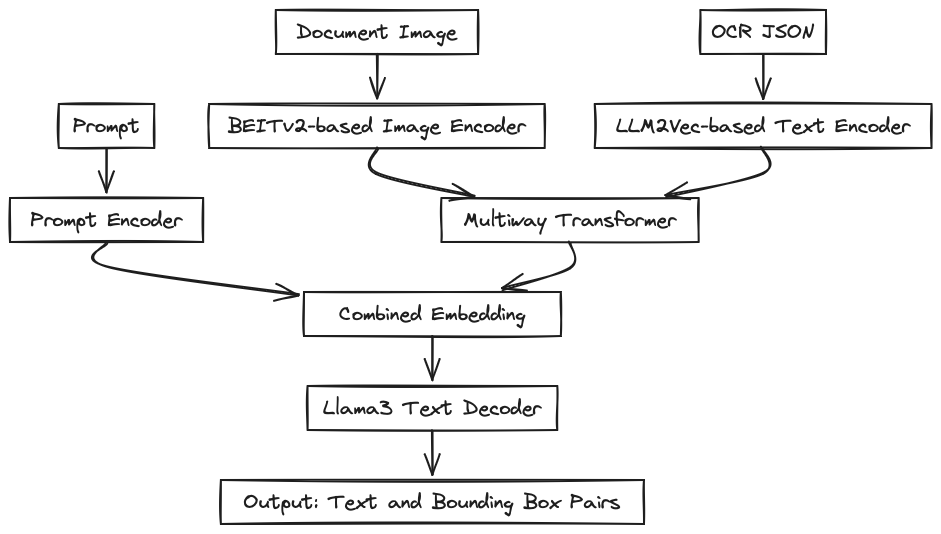
\includegraphics[width=\linewidth]{foundational_model.png}
    \caption{Foundational Model for Intelligent Document Processing}
    \label{fig:foundational-model}
\end{figure}

\textbf{Advanced Image and Text Encoding}: Our model leverages a Vision Transformer (ViT) with BEITv2 pre-training to enhance image understanding by predicting CLIP embeddings. For text encoding, we adapt a pre-trained Large Language Model (LLM) using the LLM2Vec approach, incorporating bidirectional attention, masked next token prediction (MNTP), and unsupervised contrastive learning (SimCSE). This dual approach ensures the model can handle structured OCR outputs effectively, providing a robust foundation for further processing.

\textbf{Extended Context Handling and Integration}: We incorporate LongLoRA, combining Shifted Sparse Attention (S2-Attn) and parameter-efficient fine-tuning, to significantly extend the context window without a proportional increase in computational resources. This extended context is integrated with a multiway transformer, allowing efficient cross-modal attention and enhancing the model's understanding of visual and textual relationships. This integration ensures that the model can process and understand documents with complex layouts and extended text sequences.

\textbf{Robust Pre-training, Fine-tuning, and Interaction Mechanisms}: Our model undergoes extensive pre-training on large datasets and is fine-tuned on specific tasks such as document classification, layout analysis, and named entity recognition. This fine-tuning ensures robust performance across various downstream tasks. Additionally, we incorporate a prompt encoder and text decoder, which allows the model to generate relevant answers based on given prompts and document OCR pairs. This capability enhances the model's ability to perform contextually aware information extraction, making it versatile and adaptable for various applications.


By integrating these advancements, our multi-modal foundation model is equipped to handle large context sizes efficiently, enabling it to perform well on various downstream tasks such as document classification, named entity recognition, and more. This work sets a new standard for processing multi-modal documents with extended contexts, demonstrating the powerful synergy of modern NLP and computer vision techniques.

\section{Methodology}

\subsection{Dataset Details}

\textbf{IDL-WDS:} \\
The IDL-WDS (Industry Documents Library - Web Dataset) is a comprehensive dataset designed to facilitate robust pre-training on a diverse range of document types and structures. It comprises approximately 19 million pages, including PDF files, TIFF images, and JSON files with Textract OCR annotations. For processing, images are converted to 1024x1024 pixels in TIFF format to ensure high-quality input data. OCR JSON files are parsed to extract word bounding boxes and text, with bounding box coordinates normalized relative to the 1024x1024 image size. The \texttt{litdata} library from Lightning-AI is utilized for efficient data processing, supporting data loading, transformation, and batching, optimizing the pipeline for large-scale datasets.

\textbf{PDFA-ENG-WDS:} \\
The PDFA-ENG-WDS dataset focuses on English PDF documents, providing OCR annotations and bounding boxes for words. Spanning approximately 1.5TB, it contains over 26 million pages and 18 billion text tokens. The dataset is stored in \texttt{.tar} files, compatible with efficient streaming and processing using the \texttt{litdata} library. Text and bounding box coordinates are normalized relative to the 1024x1024 image size and converted to a suitable format for model input. The \texttt{litdata} library supports efficient loading of large, sharded datasets, enabling parallel processing and handling large-scale data effectively.

\textbf{PubTables-1M:} \\
The PubTables-1M dataset is designed for table detection and structure recognition within documents, providing an extensive collection of annotated data to pre-train and fine-tune models for layout analysis and table structure extraction tasks. It includes approximately 947,642 cropped table instances and 575,305 document page instances. The dataset contains images and annotations for train, test, and validation sets, detailing table structures and word bounding boxes. Images are standardized to 1024x1024 pixels, and bounding box coordinates are normalized relative to this size. The \texttt{litdata} library is used for efficient loading, transformation, and batching of data.

\textbf{PubLayNet:} \\
PubLayNet is a large-scale dataset aimed at document layout analysis, with annotations for text, titles, lists, tables, and figures within research paper images. It contains over 1 million annotated document images sourced from PubMed Central articles. The dataset includes bounding boxes and labels for various layout components and is divided into training, validation, and test splits. Images are converted to 1024x1024 pixels, and bounding box coordinates are normalized for consistency. The \texttt{litdata} library handles large-scale data efficiently, supporting shuffling, batching, and parallel processing.

\subsection{Datasets Processing Strategy}

\begin{itemize}
    \item \textbf{Consistency:} Standardize image resolutions to 1024x1024 pixels and convert them to TIFF format to ensure high-quality, uniform input data.
    \item \textbf{Normalization:} Normalize bounding box coordinates in the OCR JSON files relative to the 1024x1024 image dimensions.
    \item \textbf{Efficient Loading:} Use the \texttt{litdata} library for data processing, \texttt{torchvision} for image handling, and efficient methods for managing large, sharded datasets. This ensures efficient data loading and processing, reducing bottlenecks during training.
    \item \textbf{Metadata Utilization:} Leverage metadata such as file sizes and rendering times to filter out large or slow-to-render files, optimizing the dataset for efficient training at scale.
\end{itemize}

By following these strategies, we can efficiently process and utilize the IDL-WDS, PDFA-ENG-WDS, PubTables-1M, and PubLayNet datasets for pre-training and fine-tuning our multi-modal foundation model, ensuring high performance across various document analysis tasks.
```

\section{Model Architecture}

\subsection{Image Encoder}

The image encoder in our model is based on the Vision Transformer (ViT) model, pre-trained using the BEITv2 approach. BEITv2 leverages a visual tokenizer to convert images into discrete visual tokens, enabling masked image modeling (MIM). Specifically, approximately 40\% of image patches are masked, and the model is trained to predict the CLIP embeddings of these masked patches. This technique ensures that the model captures high-level visual representations and is robust in understanding the visual content in documents. The pretraining also involves a [CLS] token to aggregate patch information into global representations, enhancing the model’s ability to generate comprehensive visual embeddings.

\subsection{Text Encoder}

The text encoder in our multi-modal foundation model leverages advanced techniques to handle long-context documents efficiently. We start with a pre-trained Large Language Model (LLM) such as Llama3 or Mistral and modify it to incorporate the improvements described in the LongLoRA framework. LongLoRA employs two primary enhancements:

First, \textbf{Shifted Sparse Attention (S2-Attn)} is utilized during fine-tuning to significantly reduce computational costs while maintaining performance comparable to vanilla attention. This approach ensures that the model can handle extended context lengths without a proportional increase in computational resources. Implemented with minimal code changes, S2-Attn is optional during inference, making it both efficient and flexible.

Second, \textbf{Parameter-Efficient Fine-Tuning} extends the capabilities of LoRA (Low-Rank Adaptation) by ensuring that embeddings and normalization layers are trainable. This combination enhances the model's ability to handle longer contexts effectively. Using these techniques, LongLoRA demonstrates the ability to extend the context window of LLMs substantially. For instance, Llama2 7B can be extended from a 4k context to 100k, or Llama2 70B can be extended to 32k, all while maintaining computational efficiency.

Additionally, the model with extended context capabilities is further enhanced using LLM2Vec. LLM2Vec generates high-quality contextual vector representations by leveraging the power of pre-trained LLMs and refining them for specific tasks. The process involves fine-tuning models to produce embeddings that capture the nuanced meanings of words and phrases in context. Implementing various pooling strategies, such as mean pooling, weighted mean pooling, and EOS token pooling, allows for flexible and robust extraction of sentence-level embeddings. By combining LongLoRA's extended context capabilities with LLM2Vec's advanced embedding techniques, the model is well-suited for handling large context sizes and performing well on various downstream tasks, such as document classification and named entity recognition.

The text encoder utilizes a pre-trained LLM such as Llama3 or Mistral, adapted using the LLM2Vec approach. This process includes enabling bidirectional attention, masked next token prediction (MNTP), and unsupervised contrastive learning using the SimCSE technique. The goal is to transform a decoder-only LLM into a strong text encoder. The steps involve fine-tuning the model to predict masked tokens and using dropout techniques to create positive examples for contrastive learning. This adaptation is crucial for handling the structured nature of OCR outputs, as described in "LLM2Vec: Large Language Models Are Secretly Powerful Text Encoders."

By incorporating these advancements, our text encoder is equipped to handle large context sizes efficiently, enabling it to perform well on various downstream tasks such as document classification, named entity recognition, and more.

\subsection{Integration with Multiway Transformer}

To integrate text and image embeddings, we employ a Multiway Transformer architecture. Each block consists of a shared self-attention module and a pool of feed-forward networks tailored for different modalities (vision, language, and vision-language). This design facilitates deep fusion of multi-modal data and modality-specific processing, making it highly effective for tasks involving complex interactions between text and images.

\subsection{Positional Embeddings for Bounding Boxes}

We enhance the positional embeddings to incorporate the spatial information of OCR tokens using techniques inspired by "Learnable Fourier Features for Multi-Dimensional Spatial Positional Encoding." This involves encoding the bounding box coordinates using learnable Fourier features, which capture the spatial relationships between tokens. By embedding this spatial information directly into the transformer's self-attention mechanism, the model effectively captures the topological and spatial relationships between textual elements in a document, thereby improving its performance in tasks that require an understanding of the document's visual and spatial context.

\subsection{Prompt Encoder}

The prompt encoder is a small text embedding model designed to process the prompt and generate an embedding. This embedding is then added to the embedding received from the multiway transformer before feeding into the text decoder.

\textbf{Model Architecture}:
The architecture utilizes a lightweight transformer or any efficient text embedding model for the prompt encoder. The model is designed to output embeddings of the same dimension as the multiway transformer to ensure seamless integration.

\textbf{Embedding Process}:
The process begins by taking the input prompt and converting it into token embeddings. These embeddings are then processed through the prompt encoder to generate a final prompt embedding, which is added to the multiway transformer embedding before being input to the text decoder.

\subsection{Text Decoder}

The text decoder in our multi-modal model is a fine-tuned LLM like Llama3, which generates word and bounding box pairs for various extraction tasks or plain text when describing documents.

\textbf{Model Architecture}:
We use Llama3 or another suitable LLM for the text decoder. The model is fine-tuned to handle tasks that involve generating word and bounding box pairs, as well as descriptive text for documents.

\textbf{Fine-tuning}:
The fine-tuning process involves using datasets that include document descriptions, extraction tasks, and bounding box annotations. The model is trained to generate output sequences that consist of both text and bounding box coordinates, enabling it to effectively perform various document analysis tasks.

\subsection{Integration}

The integration of our multi-modal foundation model involves combining the embeddings generated by the prompt encoder with those from the multiway transformer. This combined embedding is then passed to the text decoder. Specifically, a lightweight transformer, such as BERT, is used by the prompt encoder to convert the prompt into an embedding. This embedding is then added to the multiway transformer embedding before being input to the text decoder, typically a fine-tuned LLM like Llama3.

The training strategy for this model involves jointly training the prompt encoder and text decoder on tasks that require both text generation and bounding box prediction. This joint training approach ensures that the model can generate coherent text sequences alongside accurate bounding box coordinates. The loss function is carefully designed to account for both text and bounding box outputs, allowing the model to learn these tasks simultaneously and efficiently.

The prompt encoder processes the prompt into an embedding using a lightweight transformer model. The multi-modal model combines this prompt embedding with document embeddings from the multiway transformer, which are then passed to the text decoder. The text decoder generates the final output, producing both text and bounding box pairs for various extraction tasks. This comprehensive setup enables the model to effectively handle prompts and generate appropriate responses, ensuring it performs well on diverse document analysis tasks.

\section{Experiments}

\subsection{Pre-training Strategy and Setup}

Our pre-training strategy leverages three key objectives: Masked Language Modeling (MLM), Masked Image Modeling (MIM), and Word-Patch Alignment (WPA). Inspired by "LayoutLMv3: Pre-training for Document AI with Unified Text and Image Masking," these objectives aim to enable the model to effectively learn multimodal representations.

For \textbf{Masked Language Modeling (MLM)}, 30\% of text tokens are masked using a span masking strategy, with span lengths following a Poisson distribution. The goal is to maximize the log-likelihood of predicting these masked tokens based on contextual representations from both text and image sequences. This helps the model understand the relationship between textual content and layout information.

In \textbf{Masked Image Modeling (MIM)}, around 40\% of image tokens are masked using a blockwise masking strategy. The model is then trained to reconstruct these masked tokens using a cross-entropy loss, which encourages it to interpret visual content through the context provided by both text and image tokens. This objective ensures that the model captures high-level visual structures rather than just low-level details.

\textbf{Word-Patch Alignment (WPA)} aligns text words with their corresponding image patches. This involves predicting whether the image patches corresponding to a text word are masked. By assigning binary aligned/unaligned labels to unmasked text tokens based on their image patch masking status, the model learns a fine-grained alignment between text and image modalities, which is crucial for tasks requiring precise text-image correspondence.

\begin{enumerate}
    \item \textbf{Datasets:} We use the IDL-WDS and PDFA-ENG-WDS datasets for pre-training. These datasets provide a diverse collection of document images and corresponding OCR outputs, allowing the model to learn from various document types and structures.
    \item \textbf{Objectives:} The pre-training involves masked language modeling (MLM), masked image modeling (MIM), and word-patch alignment (WPA) objectives, ensuring the model captures comprehensive multimodal representations.
    \item \textbf{Evaluation Metrics:} We evaluate the model's performance on pre-training tasks using metrics such as cross-entropy loss for MLM and MIM, and binary cross-entropy loss for WPA.
\end{enumerate}

\subsection{Fine-tuning Strategy}

Our fine-tuning strategy adopts a prompt-based approach inspired by methods described in the Segment Anything Model (SAM). This enables the model to respond effectively to a variety of prompts tailored to solve different downstream tasks.

\textbf{Instruction Tuning the Text Decoder:} The text decoder is fine-tuned to handle diverse downstream tasks by providing specific instructions on generating the relevant output. This includes producing text sequences and identifying corresponding bounding boxes in response to various queries. By doing so, the model becomes adept at generating contextually accurate outputs based on the instructions provided.

\textbf{Zero-Shot and Few-Shot Learning:} Leveraging the model’s pre-trained capabilities, the prompt-based strategy allows it to perform tasks in zero-shot or few-shot settings. By carefully designing prompts, the model can be adapted to various applications, such as document layout analysis, document classification, and named entity recognition, without requiring extensive additional training.

This comprehensive fine-tuning strategy ensures that the model remains flexible and capable of efficiently performing a wide range of tasks. It leverages the strengths of pre-trained embeddings and prompt-based interaction mechanisms to maintain high performance across various applications.

\subsection{Evaluation Metrics}

To ensure the effectiveness and robustness of our multi-modal foundation model, we employ a variety of evaluation metrics at different stages of pre-training and fine-tuning. These metrics comprehensively assess the model’s performance.

\subsubsection{Pre-training Evaluation Metrics}

The evaluation of our pre-training strategy involves several metrics to ensure that both the image and text encoders, as well as their integration within the multi-modal framework, perform optimally.

For the \textbf{Image Encoder} based on BEITv2, we utilize three key metrics. Firstly, \textbf{Reconstruction Loss} measures how effectively the model reconstructs masked image patches using CLIP embeddings, typically evaluated through mean squared error (MSE) or cross-entropy loss. This metric assesses the model's ability to accurately recreate the visual information from the incomplete patches. Secondly, \textbf{Patch-wise Accuracy} evaluates the accuracy of predicting the correct visual tokens for the masked patches, reflecting the model's precision in understanding and completing the visual context. Lastly, \textbf{Global Representation Quality} is assessed using linear probing on a downstream image classification task, such as ImageNet, where we evaluate the model's performance through top-1 and top-5 accuracy. This metric provides insights into the overall quality of the visual representations learned during pre-training.

For the \textbf{Text Encoder} based on LLM2Vec, we focus on metrics that capture the effectiveness of language modeling and representation learning. \textbf{Masked Language Modeling (MLM) Accuracy} measures the accuracy of predicting masked tokens in the text, evaluated using cross-entropy loss. This metric indicates how well the model understands and predicts contextual information in text sequences. \textbf{Perplexity} is another critical metric, representing how well the probability distribution predicted by the model aligns with the actual distribution of the data; lower perplexity values indicate a better language model. Additionally, \textbf{Contrastive Learning Metrics}, particularly for SimCSE, include evaluating cosine similarity between positive pairs and the alignment and uniformity of the learned representations. These metrics help in understanding how effectively the text encoder captures and differentiates semantic similarities and differences.

The \textbf{Integration of the Multiway Transformer} within the multi-modal framework is evaluated through metrics that assess the alignment and retrieval capabilities of combined text and image embeddings. \textbf{Alignment Loss} measures how well the text and image embeddings are aligned, typically using cosine similarity or a similar metric. This metric is crucial for ensuring that the model effectively integrates information from both modalities. Additionally, \textbf{Cross-modal Retrieval Accuracy} evaluates how accurately the model can retrieve relevant text given an image query, and vice versa. This is assessed using metrics such as mean reciprocal rank (MRR) and normalized discounted cumulative gain (nDCG), providing a comprehensive evaluation of the model's ability to perform cross-modal retrieval tasks effectively.

These evaluation metrics collectively ensure that our pre-training strategy results in robust and efficient multi-modal representations, capable of handling a wide range of downstream tasks.

\subsubsection{Fine-tuning Evaluation Metrics}

The evaluation of our fine-tuning strategy encompasses several metrics to ensure that both the prompt encoder and text decoder, as well as their integration within the multi-modal framework, perform effectively.

For the \textbf{Prompt Encoder}, we utilize two primary metrics. \textbf{Prompt Response Accuracy} measures how accurately the prompt encoder generates embeddings that lead to correct responses from the text decoder. This is evaluated using task-specific metrics, such as the F1 score for classification tasks, ensuring that the prompt encoder provides accurate and relevant embeddings for downstream tasks. \textbf{Prompt Response Time} evaluates the efficiency of the prompt encoder in generating prompt embeddings, measured in milliseconds. This metric is crucial for understanding the real-time performance and efficiency of the prompt encoder in various applications.

The \textbf{Text Decoder} is assessed using metrics that evaluate the quality of generated text and the accuracy of predicted bounding boxes. \textbf{Sequence Generation Quality} is measured using metrics such as BLEU, ROUGE, and METEOR, which compare the generated text against reference texts to determine the accuracy and fluency of the output. \textbf{Bounding Box Accuracy} evaluates how accurately the model predicts bounding boxes, using metrics like Intersection over Union (IoU) and mean Average Precision (mAP). These metrics are essential for tasks that require precise localization and labeling of text within document images.

The \textbf{Overall Model Performance} is evaluated through task-specific metrics to ensure the model's robustness and versatility across various applications. For \textbf{Document Layout Analysis}, metrics such as F1 score, precision, recall, and mean Average Precision (mAP) are used to detect and classify different layout components, including text blocks, tables, and figures. \textbf{Document Classification} performance is measured by accuracy, F1 score, precision, and recall, ensuring that the model can accurately categorize documents into predefined classes. For \textbf{Named Entity Recognition (NER)}, the model's ability to identify and classify named entities within the text is evaluated using F1 score, precision, and recall. Lastly, \textbf{Question Answering} tasks are assessed using Exact Match (EM) and F1 score, which evaluate the correctness of the answers generated in response to specific queries.

These comprehensive evaluation metrics ensure that our fine-tuning strategy results in a robust and efficient multi-modal model capable of handling a wide range of document analysis tasks with high accuracy and performance.

\subsubsection{Evaluation during Pre-training and Fine-tuning}

During the pre-training and fine-tuning phases, continuous monitoring and evaluation are crucial to ensure that the model performs optimally and generalizes well to unseen data. One of the primary metrics used is \textbf{Validation Loss}. By continuously monitoring validation loss, we can track the model's performance and detect any signs of overfitting. This ongoing evaluation helps ensure that the model maintains its ability to generalize effectively beyond the training data.

In addition to validation loss, \textbf{Early Stopping Metrics} are employed to further prevent overfitting. Metrics such as validation loss and specific early stopping criteria, based on parameters like patience and delta values, allow us to halt training when the model's performance ceases to improve. This strategy not only helps in avoiding overfitting but also ensures efficient use of computational resources by stopping the training process at an optimal point.

Another important aspect of our evaluation strategy is conducting \textbf{Ablation Studies}. These studies involve systematically removing or altering different components of the model, such as the prompt encoder or text decoder, to assess their impact on overall performance. By understanding the contributions of each component, we can refine the model architecture and improve its robustness and effectiveness.

By utilizing these diverse evaluation metrics and strategies, we can comprehensively assess the performance and robustness of our multi-modal foundation model at each stage of pre-training and fine-tuning. This thorough evaluation process ensures that the model is well-tuned and capable of handling various downstream tasks effectively.

\section{Infrastructure for Training and Fine-Tuning}

Training and fine-tuning a multi-modal foundation model, particularly with large language models like Llama3-8B and BEITv2, and extensive datasets such as IDL-WDS and PDFa-eng-WDS, necessitates significant computational resources. Below, we outline the infrastructure requirements and the necessary setup for efficient training and fine-tuning.

\subsection{Hardware Requirements}

\begin{enumerate}
    \item \textbf{GPUs:} High-performance GPUs are essential. NVIDIA A100 GPUs are recommended, with at least 8 GPUs to handle the extensive computation and large context sizes required by models like Llama3-8B.
    \item \textbf{Memory:} A minimum of 2TB of system memory (RAM) to manage large datasets and model parameters efficiently.
    \item \textbf{Storage:} High-speed SSD storage, with at least 20TB capacity, to accommodate the large-scale datasets and model checkpoints.
    \item \textbf{Networking:} High-bandwidth networking (e.g., InfiniBand) to ensure fast data transfer between GPUs and storage, reducing bottlenecks.
\end{enumerate}

\subsection{Software Requirements}

\begin{enumerate}
    \item \textbf{Frameworks:} PyTorch for deep learning, with PyTorch Lightning to streamline the training and fine-tuning process.
    \item \textbf{Libraries:}
    \begin{itemize}
        \item \texttt{Hugging Face Transformers} for model implementations and tokenizers.
        \item \texttt{CUDA}, \texttt{cuDNN}, \texttt{xFormers}, \texttt{pyCUDA} and \texttt{triton} for GPU acceleration.
        \item \texttt{Apex} for mixed precision training to optimize performance and memory usage.
    \end{itemize}
    \item \textbf{Data Management:} \texttt{LitData} library for efficient data loading and preprocessing, particularly useful for handling large datasets.
\end{enumerate}

\subsection{Training and Fine-Tuning Environment}

\begin{enumerate}
    \item \textbf{Distributed Training:} Utilize distributed training strategies, such as data parallelism and model parallelism, to efficiently leverage multiple GPUs.
    \item \textbf{Mixed Precision Training:} Use mixed precision training to reduce the memory footprint and increase computational speed, crucial for handling large models like Llama3-8B.
    \item \textbf{Hyperparameter Tuning:} Implement automated hyperparameter tuning frameworks (e.g., Optuna or Ray Tune) to optimize model performance.
    \item \textbf{Monitoring and Logging:} Set up robust monitoring and logging systems (e.g., TensorBoard, Weights \& Biases) to track training progress and performance metrics.
\end{enumerate}

\subsection{Tooling for Reproducible Model Development}

Ensuring reproducibility in model development is crucial for validating results and facilitating collaboration. The following tools and practices are recommended:

\begin{enumerate}
    \item \textbf{Version Control:} Use Git for version control of code, configuration files, and documentation. Maintain clear commit messages and branching strategies (e.g., GitFlow).
    \item \textbf{Environment Management:} Use Docker to create isolated and reproducible environments. Document the dependencies and environment setup steps in a \texttt{Dockerfile} or \texttt{docker-compose.yml}.
    \item \textbf{Experiment Tracking:} Utilize tools like MLflow or Weights \& Biases to track experiments, including hyperparameters, training configurations, and results. This ensures that all experiment details are recorded and can be reproduced.
    \item \textbf{Automated Testing:} Implement automated tests for different components of the model pipeline using frameworks like \texttt{pytest}. This includes unit tests, integration tests, and regression tests to ensure that changes do not introduce errors.
    \item \textbf{Continuous Integration/Continuous Deployment (CI/CD):} Set up CI/CD pipelines using tools like GitHub Actions or Jenkins to automate testing, building, and deploying models. This ensures that every change is automatically tested and can be deployed consistently.
    \item \textbf{Documentation:} Maintain comprehensive documentation for the codebase, including installation instructions, usage examples, and API references. Tools like Sphinx can help generate documentation from docstrings and comments in the code.
\end{enumerate}

\subsection{Summary of Training and Fine-Tuning Process}

\begin{enumerate}
    \item \textbf{Pre-training:}
    \begin{itemize}
        \item Utilize large datasets (IDL-WDS with approximately 70 million pages and PDFa-eng-WDS with extensive document images and text pairs) to pre-train the image encoder with BEITv2 and the text encoder with LLM2Vec.
        \item Implement LongLoRA for efficient context extension, which is crucial given the extended context requirements of up to 100k tokens for Llama2 7B and 32k tokens for Llama2 70B.
    \end{itemize}
    \item \textbf{Fine-Tuning:}
    \begin{itemize}
        \item Apply a prompt-based fine-tuning strategy inspired by SAM.
        \item Fine-tune on specific datasets like PubTables-1M and PubLayNet, which provide high-quality annotated data for tasks such as document layout analysis and entity recognition.
        \item Instruction tune the text decoder to handle diverse downstream tasks and respond to various prompts, ensuring robust and flexible performance.
    \end{itemize}
    \item \textbf{Evaluation:}
    \begin{itemize}
        \item Continuously evaluate the model's performance using benchmarks and iteratively refine prompts and tuning parameters.
        \item Implement zero-shot and few-shot learning to assess model adaptability and performance on unseen tasks, leveraging the model's extensive pre-training and fine-tuning.
    \end{itemize}
\end{enumerate}

By following this comprehensive setup, the training and fine-tuning processes are optimized to handle the complexity and scale of the multi-modal foundation model, ensuring robust performance across various applications.

\section{References}

\begin{enumerate}
    \item \href{https://huggingface.co/datasets/pixparse/idl-wds}{Industry Documents Library}
    \item \href{https://huggingface.co/datasets/pixparse/pdfa-eng-wds}{PDF Association dataset}
    \item \href{https://huggingface.co/datasets/bsmock/pubtables-1m}{PubTables-1M}
    \item \href{https://huggingface.co/datasets/creative-graphic-design/PubLayNet}{PubLayNet}
    \item Bao et al., "Image as a Foreign Language: BEIT Pretraining for All Vision and Vision-Language Tasks", 2022.
    \item Liu et al., "BEIT V2: Masked Image Modeling with Vector-Quantized Visual Tokenizers", 2022.
    \item Gao et al., "SimCSE: Simple Contrastive Learning of Sentence Embeddings", 2021.
    \item "LayoutLMv3: Pre-training for Document AI with Unified Text and Image Masking", 2022.
    \item "LongLoRA: Efficient Fine-Tuning of Long-Context Large Language Models", OpenReview 2023.
    \item "LLM2Vec: Enhancing Large Language Models with Contextual Vector Representations", 2024.
    \item "Learnable Fourier Features for Multi-Dimensional Spatial Positional Encoding", 2021.
    \item "MosaicBERT: A Bidirectional Encoder Optimized for Fast Pretraining", 2023.
    \item "The Power of Scale for Parameter-Efficient Prompt Tuning", 2021.
\end{enumerate}

\end{document}





